%# -*- coding: utf-8-unix -*-
%%==================================================
%% chapter01.tex for SJTU Master Thesis
%%==================================================

%\bibliographystyle{sjtu2}%[此处用于每章都生产参考文献]
\chapter{基于查询系统的知识图设计}
\label{chap:c6}
\section{背景知识}
知识图谱是将知识整合后以图的形式表现的一种方法,也是一种可视化的知识管理工具。在毕设开题报告的时候,我就一直思考如何为我的偏工程的设计中发掘出一些理论意义,于是便有了这个结合查询系统进行知识图设计的想法。该功能的构想基于如下考量:用户使用学术网站进行查询的时候,可能只重点关注搜索结果的前几条,而隐藏在大量搜索结果之中的信息则无法很好的被用户知晓。论文希望设计出一套根据用户输入的查询关键词动态生成知识图,帮助用户发掘出这些埋藏的信息。例如对于用户可能对“节能”这一关键词感兴趣,于是他键入这一关键词并查询,系统则能在环境科学、经济学、电气、化学、数学等领域梳理出相关研究的层级状知识图,以帮助用户更好地确定与了解自己的研究方向。

\begin{figure}[!htp]
  \centering
  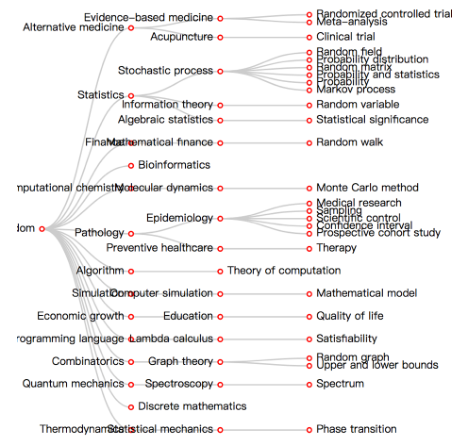
\includegraphics[width=0.6\textwidth]{knowledgegraph.png}
  \bicaption[fig:knowledgegraph]{一个简单的层级状知识图}{一个简单的层级状知识图}{Fig.}{A simple layered knowledge graph}
\end{figure}

为了更好地说明我的设计目标,我绘制了一个简单的层级状知识图作为示例。为了插图易于阅读,我们隐去了最高层L0层级,避免知识图过于复杂。如图所示,对于用户输入的关键词random,我们可以看到几棵规模较大的子树,例如Alternative Medicine(替代医学),Statistics(统计学),Pathology(病理学)等;也有一些规模不大但是我个人比较感兴趣的子树,例如Algorithm(算法)和Programming Language(编程语言)等;同时,还有Quantum Mechanics(量子力学)等重要的学科子树。这些子树又扩展开,给我们展示了这些领域的子领域相关知识。

此图是基于用户搜索random这一关键词,根据查询结果动态生成的。显然,该图相比单纯的查询结果列表能反映出更多的信息。例如,“随机”这一关键词在医学领域的应用比在计算机领域要更加地广泛,并且和统计学密切相关。如果一个研究者对“随机”这一关键词感兴趣,他如果作为一名应用科学的从业者,那么可以更多的了解到理论科学方面统计学的相关的知识点,并作为自己的研究工具;如果他是一名理论科学的从业者,也可以通过了解到随机这一关键词在医学与计算机科学方面的应用,从而给自己理论的实际应用带来灵感。这就是根据用户搜索的内容来动态生成知识图的应用。目前的主流学术网站上很少有与该设想相重复的功能,这也是我继续这一研究的一大动力。

在理论方面,有很多的论文为我研究这一问题起到了很大的启发作用。Ronen Feldman的文章\citen{mtukd}介绍了根据实体的关键词分布进行数据挖掘的各种算法,为如何从理论的角度量化研究论文的关键词信息提供了很大的启发;Hsin-Ning Su的论文\citen{mksbk}介绍了从关键词的共现性绘制知识结构的方法,并讨论了该方法在二维知识图绘制中的应用;Yuefeng Li的论文\citen{mofaa}通过分析关键词的相关性和非相关性给出了关键词信息的筛选手段,对我们的图规模控制算法起到了启发作用;Stanley Loh的论文\citen{cbkdi}给出了关键词相关性的置信度算法,为我们对关键词之间相关性的计算给出了启发。

有了这些理论基础,我们就可以从最简单的层级状知识图入手设计我们的动态知识图生成功能。

\section{知识图生成基础算法}
与背景知识的示例中一样,我们利用查询结果中的论文关键词信息绘制层级状知识图。在这里,本文章的第4.2章中介绍的结果统计功能(facet)恰好能为我们所用。结果统计功能恰好统计了论文的关键词信息,其基本结构如下:
\begin{lstlisting}[caption={关键词结果统计}, label=kwfacet, escapeinside="", numbers=none]
{
"facet\_counts":{
    "facet\_queries":{},
    "facet\_fields":{
      "PaperPublishYear":[.....],
      "KeywordID":[
        "017C8A77",9940,
        "08EE83EF",5945,
        "09AEBB9C",4648,
        "200524E7",4165,
        .....],
      .....},
    "facet\_ranges":{},
    "facet\_intervals":{},
    "facet\_heatmaps":{}}
}
\end{lstlisting}

其中,KeywordID虽然用不直观的十六进制字符串的形式表示,但是在数据库中能很方便的查询到ID对应的实际内容,经过转化后如下:
\begin{lstlisting}[caption={关键词结果统计\_新}, label=kwfacet2, escapeinside="", numbers=none]
{
    "KeywordID":[
      "Water content",9940,
      "Chemical composition",5945,
      "Content analysis",4648,
      "Nitrogen",4165,
      .....]
}
\end{lstlisting}

在此图中我们便可以很明确地看到关键词结果统计的详细信息,我们的查询语句为“content”,而查询结果论文拥有关键词排名的前几名都与化学成分分析等领域密切相关。上表也正是一张包含了“content”这一单词的论文的关键词出现频率的排行榜。

我们的数据库中还有一张记录了关键词之间层级关系的表,它记录了每个在论文中出现过的关键词,其所在的层级(L0, L1, L2, L3)与关键词的父关键词,其中L3为最细分的层级,而L0为最概括的层级。结合这张表的内容,我们即可以实现知识图生成的基础算法。首先,我们说明如何生成一颗基础的树状知识图:

\begin{algorithm}
% \begin{algorithm}[H] % 强制定位
\caption{生成基础的树状知识图}
\label{getrawtree}
\begin{algorithmic}[1] %每行显示行号
\Ensure 树状知识图$knowledgetree$ % 输出
\Require 用户查询关键词$userinput$, 结果统计关键词列表$keylist$, 关键词层级关系表$hierarchy$ % 输入
\State $knowledgetree \gets \{\}$
\State $root \gets userinput$
\State $knowledgetree.append(root)$
\For{$node$ in $keylist$}
  \State $node.parent \gets hierarchy[node]$
  \If {$node$ not in $knowledgetree$ and $node.parent==None$}
    \State $node.parent \gets root$
    \State $knowledgetree.append(node)$
  \EndIf
  \If {$node$ not in $knowledgetree$ and $node.parent != None$}
    \State $nodep \gets node.parent$
    \State $knowledgetree.append(node)$
    \State $keylist.append\{nodep\}$
  \EndIf
\EndFor
\end{algorithmic}
\end{algorithm}

通过该算法,我们可以得到得到一棵理论上信息完全的知识图树结构,但是其保存的数据结构还略显混乱,因此我们需要进一步将之前得到的数据结构进行格式化。一个好的树的数据结构应该是这样的:

\begin{lstlisting}[caption={树数据结构}, label=treestructure, escapeinside="", numbers=none]
{node:{
  nodeproperty1 : aaa,
  nodeproperty2 : bbb,
  ...,
  children:{node*}
  }
}
\end{lstlisting}

在该数据结构中,树用一个字典进行表示,字典中只有一个键为根节点的元素,其值为根节点的各种属性与子节点列表。子节点字典要么为空,要么包含的元素递归地为与根节点相同的字典结构。

上述优结构的树与算法6-1得到的树最大的区别在于,优结构树中父节点总是在子节点之前出现的,而算法6-1得到的树的父节点会经常地在子节点之后出现。可以运用递归函数,用栈的思想即可将算法6-1得到的输出转化为上述优字典结构的树。具体实现此处略去。

得到了优结构的树后,我们即可以开始考虑知识图的绘制问题。

\section{知识图的绘制}
我们使用数据可视化工具d3.js来进行知识图的绘制。d3是数据驱动文档(Data Driven Document)的简称,它以开源Javascript代码的形式提供了很多方便的网页数据可视化接口。d3.js提供了许多绘制层级状树结构的示例接口。例如图6.1的系统树图(Dendrogram),下图所示的径向树(Radial tree)与放射图(sunburst)等。

\begin{figure}[!htp]
  \centering
  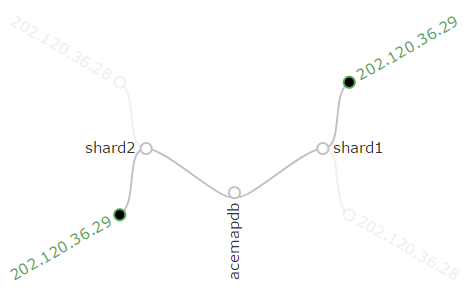
\includegraphics[width=0.3\textwidth]{radial.png}
  \hspace{1cm}
  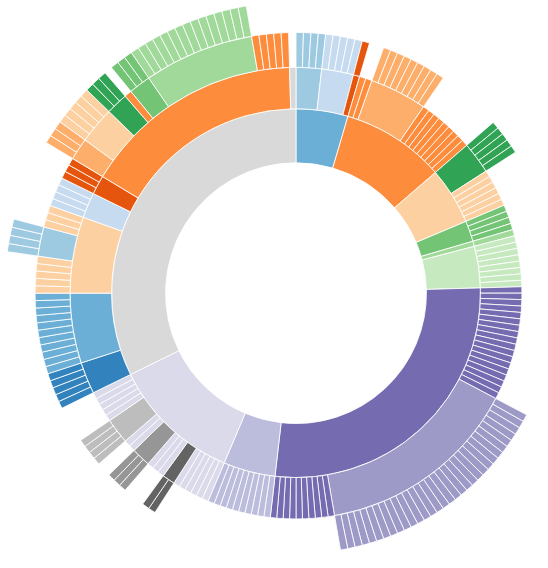
\includegraphics[width=0.3\textwidth]{sunburst.png}
  \bicaption[fig:sunburst]{径向树与放射图}{左:径向树;右:放射图}{Fig}{radial tree and sunburst}
\end{figure}

这些工具都可以用来展示层级状知识图,但是以上两幅图相比图\ref{fig:knowledgegraph}的传统树状图,对空间的利用率更高,且支持更多的用户交互动作,因此更适合在网站中使用。运用这些接口绘制我们的我们的层级状知识图,图上的圆心代表用户查询的关键词,而图上的同心圆从内到外依次代表树节点各层次的内容 。实际绘制得到的效果如图\ref{fig:sunburst2}所示。

\begin{figure}[!htp]
  \centering
  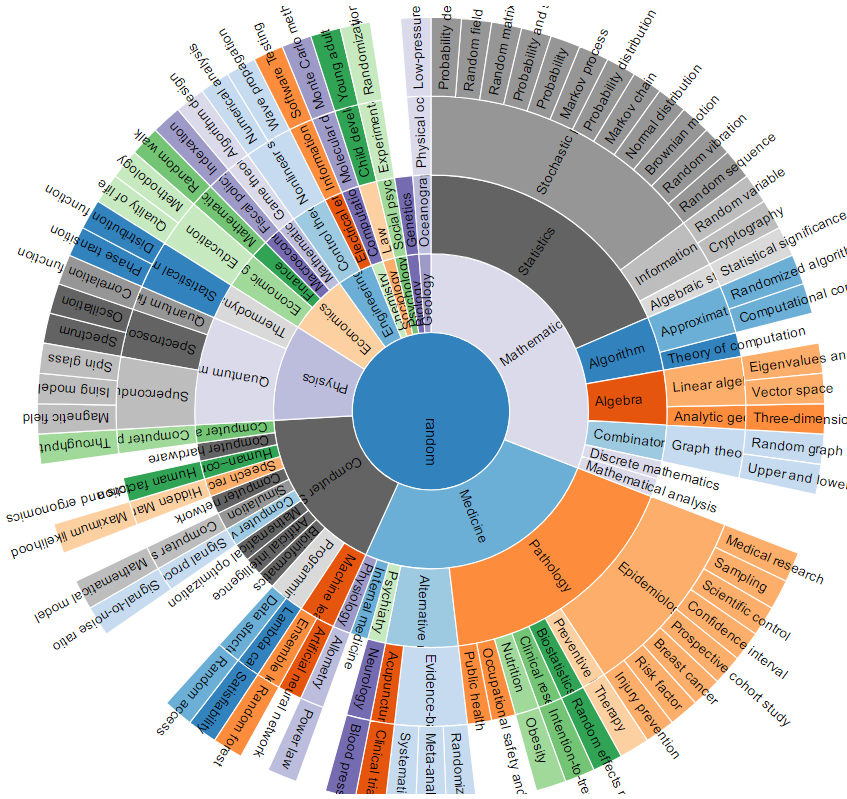
\includegraphics[width=0.45\textwidth]{sunburst2.png}
  \hspace{1cm}
  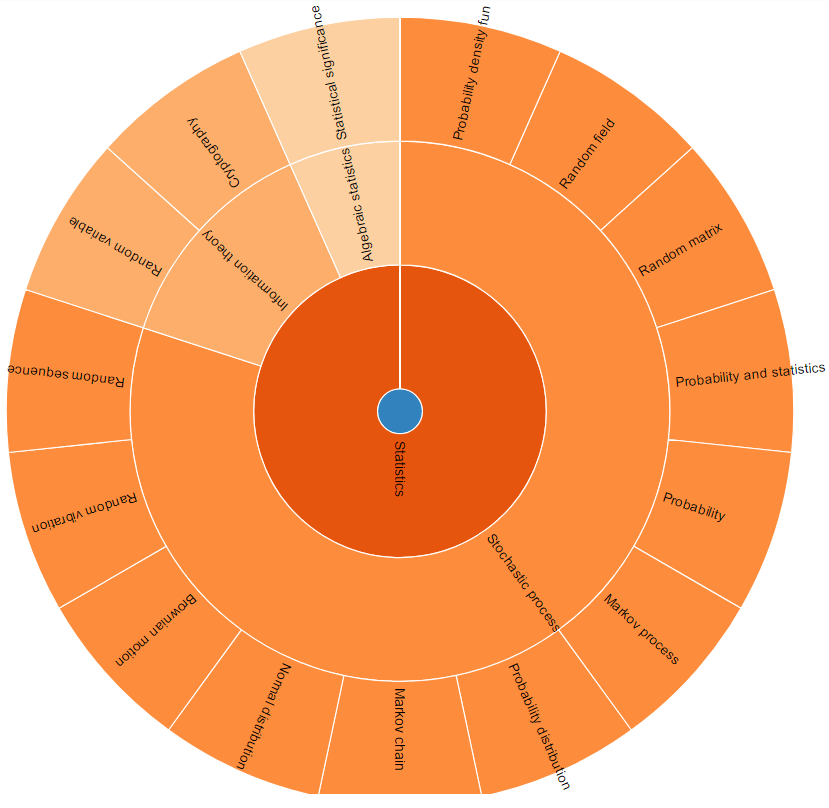
\includegraphics[width=0.45\textwidth]{sunburst3.png}
  \bicaption[fig:sunburst2]{放射状知识图与知识图子树}{左:放射状知识图;右:知识图子树}{Fig}{sunburst and subtree sunburst}
\end{figure}

图\ref{fig:sunburst2}中左图是算法6-1得到的树结构化后直接绘制的知识图,右图是将左图两点钟方向的子树放大后的效果。可以看出,绘制的知识图已经有了初步的雏形与信息量,但是也存在着明显的问题。左图包含的节点数显然过多,左上角部分有大量紧密的难以阅读的节点;而右图包含的节点数又太少,使得放射图的表现效果不佳。因此,下一步我们需要进行知识图的规模控制,将知识图的节点数控制在一个合适的水平。

\section{知识图规模的控制}
我们用以下算法流程实行知识图规模的控制:
\subsection{去除信息缺失的节点}
我们生成的知识图以树的形式呈现,其中树的根节点是人为加入的参考节点。去除根节点,可以得到一组树${T_1,T_2,...,T_n}$。这些树中的节点均为论文的关键词节点,节点包含层级信息${L_0,L_1,L_2,L_3}$,代表关键词节点在论文关键词层级表中处于哪一层。考虑图\ref{fig:sunburst2}中的左半部分,其中包含了一些直接连接至根节点的$L_2,L_3$层节点,它们同时也是子树集合${T_1,T_2,...,T_n}$的根节点。我们认为,直接连接至根节点的$L_2,L_3$层节点处于较为细化的层次,其子节点层数至多为一层,且很有可能是因为数据库信息缺失导致的父节点信息丢失。这些信息缺失的节点会影响对整张图层级化结构的认识,因此我们将这些节点联通其连接的树结构删去。详见算法\ref{ago1}。

\begin{algorithm}
% \begin{algorithm}[H] % 强制定位
\caption{去除信息缺失的节点}
\label{ago1}
\begin{algorithmic}[1] %每行显示行号
\Ensure 子树集合$\{T_1',T_2',...T_m'\}$ % 输出
\Require 原始树集合$\{T_1,T_2,...T_n\}$ % 输入
\For{$t$ in $\{T_1,T_2,...T_n\}$}
  \State $troot \gets t.root$
  \If {$troot.layer==L2$ or $troot.layer==L3$}
    \State remove $t$ from $\{T_1,T_2,...T_n\}$
  \EndIf
\EndFor
\end{algorithmic}
\end{algorithm}

\subsection{计算节点的规模值}
在这一部分中,我将描述如何进一步地选取知识图中相对更为重要的节点。此处,我们采用一维Kmeans聚类\citen{kmeans}的方法选取规模值最大,也就是重要度最高的一系列节点,并将其它节点删去,从而控制整棵树的规模。在此算法构思的形成上,我们受到了文献\citen{topic}和\citen{keyword}中的对关键词进行聚类的算法的启发,但是并没有照搬文献中的公式,而是针对我们自己的问题用类似的思想构建了一套自己的公式。

本算法中用到的符号定义如下:

\begin{longtable}{rl}
$L_{i}$: 		& 关键词处于的层次; \\
$T_{L_{i},j}^{Q}$:     & 以第$L_{i}$层的第$j$个节点为根节点,$Q$为根节点父节点的子树; \\
$S(T)$:     & 子树的规模值,此处及以下的T均为$T_{L_{i},j}^{Q}$的简写形式; \\
$N(T)$:     & 子树的权重值; \\
$D(T)$:     & 子树根节点所在的深度值,即$L_{i}$中的i值加上1; \\
$F(T)$:     & 子树根节点在$Q$的所有子节点中的重要度; \\
$f(T)$:     & 子树根节点出现频率; \\
$f_{max}$:     & $Q$的子节点的最大出现频率; \\
$f_{min}$:     & $Q$的子节点的最小出现频率; \\
$m_{T}$:     & 传递系数 \\
\end{longtable}

算法的中心思想,即为根据节点的相关信息计算出子树的规模值$S(T)$,之后对子树的规模进行聚类,保留规模较大的聚类,而删除规模较小的聚类,从而达成了知识图的规模控制效果。其中,子树规模值$S(T_{L_{i},j}^{Q})$的计算公式如下:

\begin{equation}
S(T_{L_{i},j}^{Q})=\sum_{k=1}^{n}m_{T_{L_{i+1},k}^{Q'}}\cdot S(T_{L_{i+1},k}^{Q'})+N(T_{L_{i},j}^{Q})
\end{equation}

其中,k从1到n遍历了子树T的根节点的所有子节点。该算法是一个递归算法,算法基于如下考量:对于任意一个子树$T$,只要该子树含有多余一个节点,那么删去该子树的根节点,可以得到一个树的集合${T'_1,T'_2,...,T'_m}$。我们采用递归算法,认为子树$T$的规模值为上述树集合中所有树的规模值乘以传递系数并求和,加上该子树本身的权重值。如果子树$T$本身已经是叶子节点,那么前一项的值为0,直接用该节点的权重值代替节点的规模值。$m_{T_{L_{i+1},k}^{Q'}}$为比例系数,其代表节点$T_{L_{i+1},k}^{Q'}$是否在搜索统计结果里直接出现。如果直接出现则该比例系数为1,否则该比例系数为0。

接下来,我们定义节点的权重值$N(T_{L_{i},j}^{Q})$。权重值的定义方式如下:

\begin{equation}
N(T_{L_{i},j}^{Q})=(\alpha_1\cdot f(T_{L_{i},j}^{Q}) + \alpha_2\cdot\frac{1}{D(T_{L_{i},j}^{Q})})\cdot F(T_{L_{i},j}^{Q})
\end{equation}

\newpage

其中,$f(T_{L_{i},j}^{Q})$指树$T_{L_{i},j}^{Q}$根节点的出现频率,该值在查询系统的统计结果中可以得到。$D(T_{L_{i},j}^{Q})$是指树$T_{L_{i},j}^{Q}$根节点的深度,也就是$L_{i}$中的$i$值加上1。$\alpha_1$,$\alpha_2$为比例系数,我们取$\alpha_1=\frac{1}{\max_{i=1}^N(f_i)}$,$\alpha_2=1$。

$F(T_{L_{i},j}^{Q})$子树根节点在$Q$的所有子节点中的重要度,其计算公式为:

\begin{equation}
F(T_{L_{i},j}^{Q})=\frac{f(T_{L_{i},j}^{Q})-f_{min}}{f_{max}-f_{min}}
\end{equation}

注意$f_{max}$与$\max_{i=1}^N(f_i)$的区别。$f_{max}$是拥有同一父节点的所有子节点的频率值的最大值,$\max_{i=1}^N(f_i)$是图中所有节点的频率值的最大值。

运用以上公式,即可计算出所有节点的规模值。

\subsection{选取规模值最大的节点聚类}

在上一节中,我们阐述了节点规模值的计算公式。节点规模值同时考虑了三个要素,一是节点的子节点的规模值会被传递到父节点,二是节点的深度值和包含论文的数量会影响到节点的重要性,三是节点与兄弟节点包含论文的相对数目会影响到节点的取舍。

在计算了节点规模值后,我们即需要确认哪些节点需要保留,而哪些节点不需要保留。我们的计算方式是按层计算,即当内层的计算结束,节点过滤工作完成后,我们才会开始计算外层的节点取舍。在节点取舍上,我们采用了kmeans聚类的算法。我们将同层的节点按规模值聚类为重要和不重要两类,并保留分类为重要的所有节点,删除分类为不重要的所有节点及其所有的子节点。

选用kmeans算法而不选用贪婪法的原因在于节点选择的公平性。例如当某层节点的规模值依次为{3,3,5,5,5}时,我们倾向于保留三个规模值为5的节点,而当节点的规模值一次为{3,3,3,5,5}时,我们则倾向于只保留两个规模值较大的节点。而这种动态的节点保留思想,用kmeans算法可以得到很好的体现。该算法的描述如下:

\begin{enumerate}
\item 取a,b初始值a=0,b=1;
\item 计算所有节点的规模值到a,b的距离,即与a,b分别做差的绝对值。与a较近的节点标记为A,与b较近的标记为B;
\item 将标记为A的所有节点规模值的平均值作为新的a,标记为B的所有节点规模值的平均值作为新的b,重复第2,3步操作,直到集合A,B内的元素不改变为止;
\item 返回集合A,B。
\end{enumerate}

最后,我们将集合B中的节点作为保留节点,集合A中的节点作为被过滤的节点,即达成算法目标。

\section{知识图的显示效果}
我们运用以上算法保留重要度相对较高的节点,并删除了一些重要性相对较低的节点,目的就是把最终知识图的规模控制到合理的范围内。因为是动态生成层级状知识图的算法,所以我们没有采用高复杂度的算法,而是更加重视算法在系统上的响应速度,以保证该功能可以顺利上线。经过测试,本方法在知识图的规模控制上有着很好的效果。为了进一步丰富展示的内容,我们用放射图圆弧的弧度直观显示对应关键词的对应论文数目,并将论文数量随年份的演化关系在图右侧的折线图上显示。最终的显示效果如图\ref{fig:sunburst4}所示。

\begin{figure}[!htp]
  \centering
  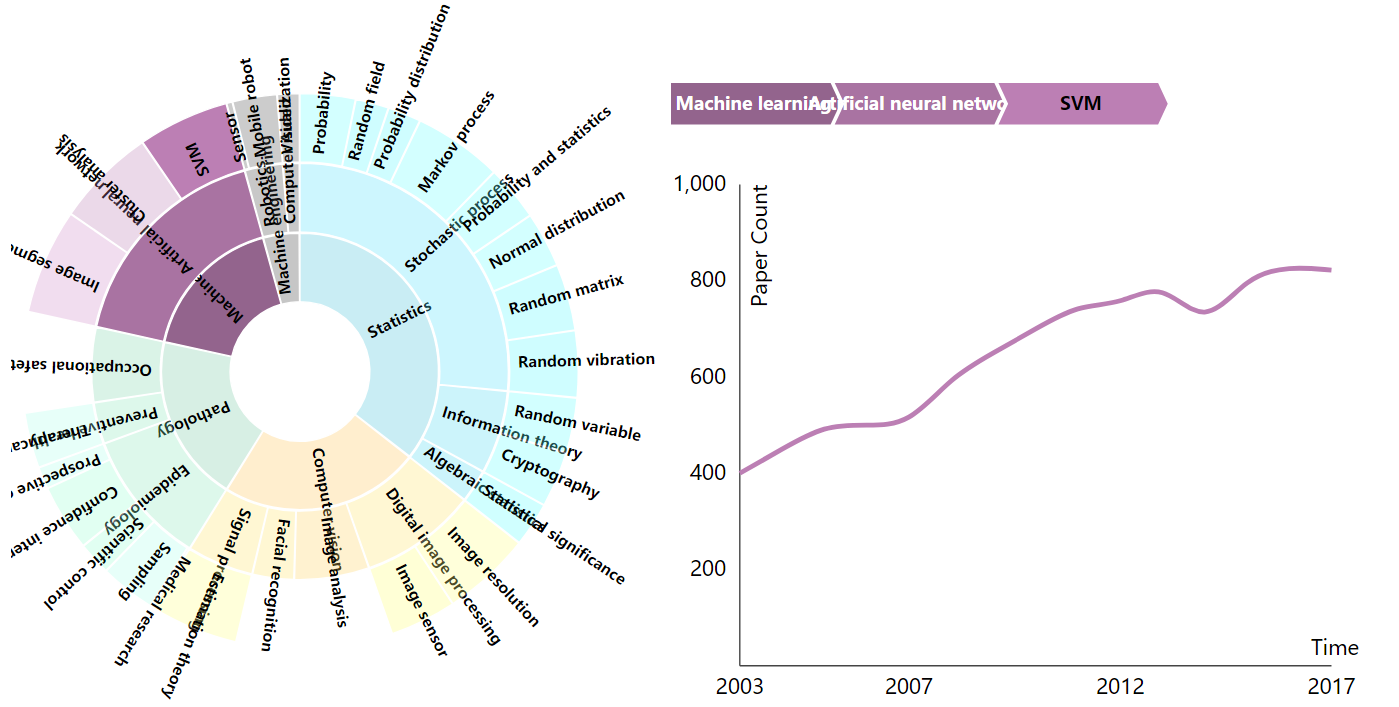
\includegraphics[width=0.75\textwidth]{sunburst4.png}
  \bicaption[fig:sunburst4]{放射状知识图最终效果}{放射状知识图}{Fig}{sunburst knowledge graph}
\end{figure}

如图,运用d3.js提供的交互式脚本我们实现了知识图的最终效果。在知识图的规模被合理化的同时,系统会跟踪用户鼠标指针的位置,并显示鼠标指向的块的层次关系和其对应的关键词论文数随时间的变化趋势。至此,基于查询系统的知识图设计功能即完成实现。